\subsection{Dialog Act and Turn Length Distribution}
\label{sec:opposite}

In Section \ref {sec:data:summary}, we reported that the relative turn length feature was giving us results opposite from what we expected.  We found that the chance of turn change is higher when the speaker has the floor for shorter than its average turn. And that the speaker will likely to keep the floor when speaking more than the average turn length. 

We suspect that the reason that our initial hypothesis proved to be incorrect is due \ph{add: to} structural properties of the corpus. \ph{was: `I.e. We'.  I.e. cannot start a sentence.  Plus, this is not a case where you can use i.e.} We were assuming that turn lengths would have a somewhat normal distribution.  In that case, if a partial turn was shorter than a speaker's average, the speaker would tend to keep speaking.  If it was longer than a speaker's average, the speaker would tend to stop speaking.

\begin{figure}[ht!]
\centering
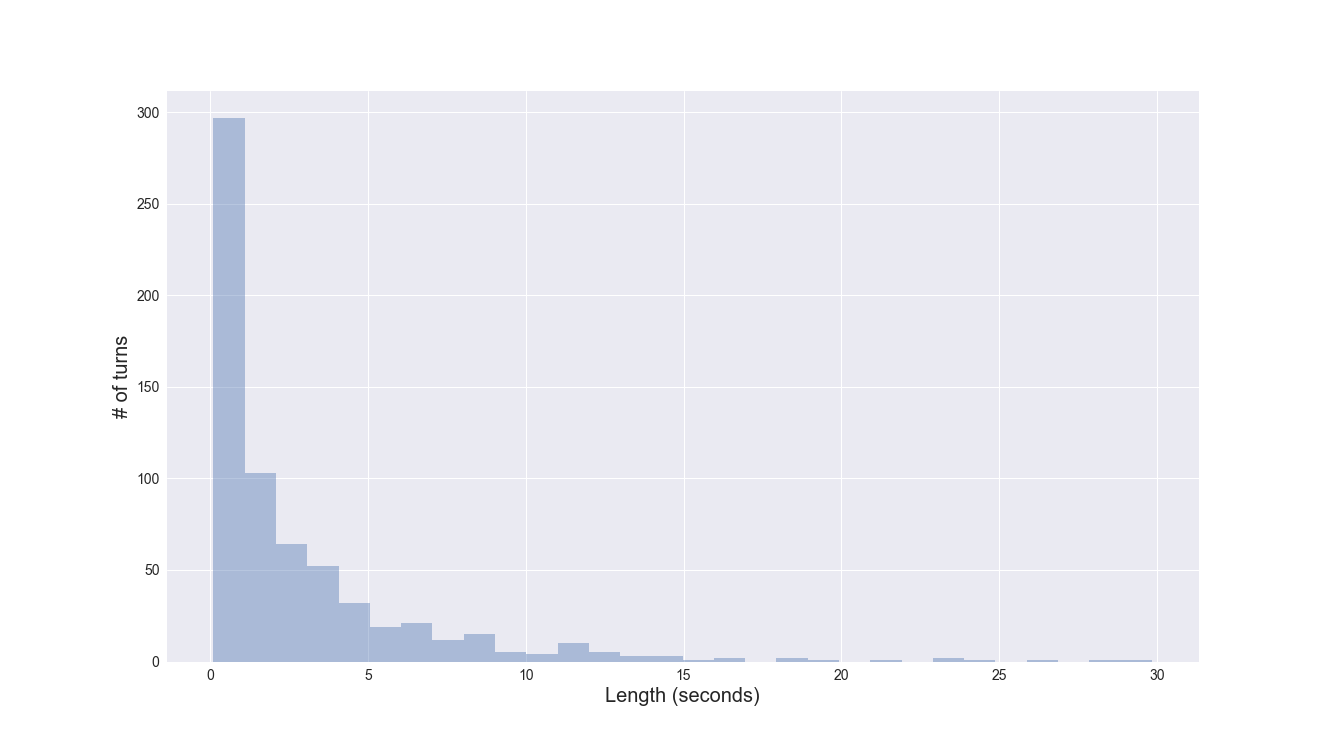
\includegraphics[width=\textwidth]{../scikitlearn/figures/f10.png}\vspace{-1em}
\caption{Distribution of the turn length}
\label{fig:turn_dist}
\end{figure}
%
Figure \ref {fig:turn_dist} shows the actual distribution of turn lengths (in seconds).
We see that the distribution of turn length is highly skewed toward short turns (back channels, short answers). Having a \ph{was: skew}skewed distribution resulting in relative short average turn length (2.88 secs), which \ph{was: cause}causes either low RTL values for short turns, or very high RTL numbers when the speaker uses a statement, or long answer. The \ph{was: results}result is that turn \ph{was: transition}transitions occur at very short turns (with relative turn length less than 100\%). Note that this figure is not directly comparable to Figure \ref {fig:rtl:turn} as that figure is realized for each speaker, allowing it to take into account speaker differences.
\phcomment{This is a pretty shallow analysis.  My hope is that you could explain why for very small RLT, odds of turn-change are high, and why if you have a high RLT you have a low odds of turn-change.  I think this might be due to how many samples are very early.  That is why I asked you how many turns are there in the data from figure 4.9?  I bet that more than half the samples are in the first histogram.  Also, I think the curve has a very flat tail, which makes high values of RLT have low odds of turn-change.  I cannot write this, as this is your thesis.  I think this analysis would be useful in understanding your RTL feature}




